%
% File acl2015.tex
%
% Contact: car@ir.hit.edu.cn, gdzhou@suda.edu.cn
%%
%% Based on the style files for ACL-2014, which were, in turn,
%% Based on the style files for ACL-2013, which were, in turn,
%% Based on the style files for ACL-2012, which were, in turn,
%% based on the style files for ACL-2011, which were, in turn, 
%% based on the style files for ACL-2010, which were, in turn, 
%% based on the style files for ACL-IJCNLP-2009, which were, in turn,
%% based on the style files for EACL-2009 and IJCNLP-2008...

%% Based on the style files for EACL 2006 by 
%%e.agirre@ehu.es or Sergi.Balari@uab.es
%% and that of ACL 08 by Joakim Nivre and Noah Smith

\documentclass[11pt]{article}
\usepackage{acl2015}
\usepackage{times}
\usepackage{url}
\usepackage{latexsym}
\usepackage{graphicx}
\graphicspath{{images/}}

%\setlength\titlebox{5cm}

% You can expand the titlebox if you need extra space
% to show all the authors. Please do not make the titlebox
% smaller than 5cm (the original size); we will check this
% in the camera-ready version and ask you to change it back.


\title{Layperson Legal Query Translation}

\author{Kristin Day \\
  Indiana University \\
  Bloomington, IN \\
  %Affiliation / Address line 2 \\
  %Affiliation / Address line 3 \\
  {\tt kricrone@iu.edu} \\\And
  Nithipat Tanmanatragul \\
  Indiana University \\
  Bloomington, IN \\
  %Affiliation / Address line 2 \\
  %Affiliation / Address line 3 \\
  {\tt ntanmana@umail.iu.edu} \\\And
  Jordan Reifsteck \\
  Indiana University \\
  Bloomington, IN \\
  {\tt jreifste@indiana.edu} \\ }

\date{}

\begin{document}
\maketitle
\begin{abstract}
This paper will show that lay person inquiries can be transformed into legal terminology allowing for accurate results from searches of legal statutes and judicial opinions.  Currently, meaningful searches of legal information are provided at high cost because of the manual nature of legal text indexing.  This research and related work endeavor to automate many of the processes related to legal text searches in order to produce an affordable solution that will be accessible to the public.  But, simple access is not sufficient.  The system must be reasonably understood by untrained individuals.  This research is a first step toward making legal search tools usable by laypeople who are not trained in law and are not familiar with legal vocabulary.

While other studies have been performed using tools such as Normalized Google Distance (NGD) to find word similarities, at the time of this writing the authors were not familiar with any research using Word2Vec models for word associations or ontology allignment.  This study discusses the downfalls of the NGD method and uses Word2Vec models to find word associations between layperson legal terminology and legal text terminology.
\end{abstract}

\section{Introduction}
In the United States, the citizens are held responsible for knowing and understanding the law.  As the English jurist John Seldon (1584-1654) reflected: ``Ignorance of the law excuses no man. Not that all men know the law, but because `tis an excuse every man will plead, and no man can tell how to refute him.''  Yet, even though every man is held accountable to the law, the law is not meaningfully available to the citizens of the United States.

Most citizens are woefully unaware of the lack of access to meaningful legal information in the United States.  Relying on Google searches and other online forums such as Justia.com and Findlaw.com, the average citizen is often led down a ``rabbit hole''\cite[p.~33]{Bruce2000}  of misinformation later to be disappointed by court appearances gone awry.  

The word clouds below demonstrate the differences between layperson terminology and legal text terminology:
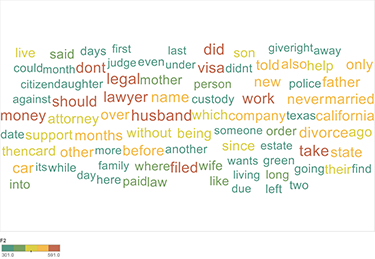
\includegraphics{UserWordCloud}

\textbf{Layperson Terminology}

\vspace{10mm}

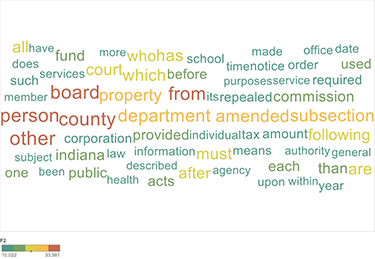
\includegraphics{StatuteWordCloud}

\textbf{Legal Text Terminology}

\subsection{Lack of Meaningful Access to Legal Information}
While there are two important access issues related to legal searches:
\begin{itemize}
\item 1) the actual unavailability of legal information to the public due to restrictions placed by the two leading legal information providers, and 
\item 2) the lack of access due to failure of understanding information that is actually available.  The former issue will be discussed in reference to the article by Melissa Barr and the latter will be discussed in reference to the article by Thomas R. Bruce.
\end{itemize}
this study focuses on the latter issue: assisting a public who does not understand legal terminology with using legal search tools.  
  
\subsection{Access Limited by Lack of Understanding}
``Public Legal Information:  Focus and Future'' by Thomas R. Bruce discusses the purpose of public libraries and other free and publicly available sources of information.  Bruce notes that with the continually increasing amount of data available, simply allowing free public access to all of that information is not sufficient to allow for public self-education.  Bruce attempts to promote an idea of providing meaningful legal information to individuals of higher than average education, or ``lay professionals.''  This implies that perhaps the average citizen, even with more advanced public legal resources, may not have sufficient skill and knowledge to aptly use legal resources.  Bruce provides the following cautionary example:

\hangindent=0.5cm
``Consider the intelligent layperson who steps up to an AltaVista or a Yahoo with question in hand and legal problem in mind.  It is not far-fetched to imagine that she could formulate a search adequate to pull up a reference to the United States Code or, better still, a Supreme Court decision.  `Aha!' she says, `that looks like the last word on my problem', and click!, she finds herself dropped like Alice down the rabbit hole into a Supreme Court opinion that seems vaguely related to her situation, but on some odd, abstract and subtly distorted plane well removed from the treatment her child has received at the hands of school authorities or the problem that her small business is having with the inspector or the tax collector.'' \cite[p.~33]{Bruce2000}

In law, more so than in other informational topics, it is easy to be misinformed or led astray by red herring cases.  And, legal misinformation can cause serious real life consequences.  Although publicly funded defense attorneys are provided to indigent criminal defendants, most legal parties must find ways to navigate the legal system without representation or pay the high price of a trained attorney.  What might be at stake in these cases?  Ownership of your home, whether you have a right to live in your rental unit, or whether or not a debt collector can levy all of the funds in your bank account.   

Although greater resources for legal information are available today than in 2000 when \cite{Bruce2000} was written, there is still a gaping divide between the requisite legal knowledge for court appearances and the information currently and meaningfully available to the public.  As \cite{Bruce2000} states so well, the systems we have in place ``are far more suited to the task of self-education in any place at any time than big buildings full of books ever were.  We can make them even better if we acknowledge that self-education is an important part of what [public libraries] are providing, and take the steps necessary to guarantee that public access is effective as well as ubiquitous.''\cite[p.~34]{Bruce2000}    It is not enough for the services of major legal data providers or public information providers to be accessible and affordable for the public; topically correct and easily understood legal information must be reasonably glean-able from the vast treasury of US legal data. 
\subsection{Goals}
This study is intended as an initial step toward making legal information meaningfully accessible to the public.  The overall goal of this and future work is to create a searchable legal database that uses layperson terminology as input and returns accurate and understandable results.  The diagram in Figure 1 shows the flow of information through the AI platform as it is envisioned.   


\includegraphics{FigFuture}

Fig.1: Illustrating proposed legal search flow

Notice that this model not only translates layperson inquiries into legal terminology to produce accurate search results, it also asks follow up questions to ensure that all of the relevant information has been collected from the user.  After the results have been retrieved from the legal database, the system will return a plain English summary with links to the legal resources to assist the user with understanding the content returned.

\section{Related Work}
Significant prior research has been done both in finding similarity distance between words and ontology alignment.  Both of these areas of study pertain to the research herein.  Although this study attempts to relate two simple lists of words (better described as lexicons than ontologies), the work related to ontology alignment applies to the outcome desired in this experiment.

\subsection{Similarity Distance}
According to \cite[p.~77]{JiangWangZheng2014}, there are two groups of similarity measures: lexical and structural.  ``The main idea in lexical measures is the fact that similar entities usually have similar names or descriptions across different ontologies.  On the other hand, the main idea in structural measures is based on considering the kinship of the components and structures residing in the ontology graphs.''  Because this study attempts to relate two simple word lists or lexicons, the focus is on measures of lexical similarity.  Although the Word2Vec model that will be utilized analyses semantic relationships of words as they appear in the context of sentences, the structure referenced in \cite{JiangWangZheng2014} refers to ontological structure as opposed to sentence structure.  

Normalized Google Distance (NGD) has been one of the primary tools used for finding similarity distance between words.  It is based on Normalized Information Distance (NID) and the Kolmogorov Complexity.  NID is a method for finding the distance between any objects.  The Kolmogorov Complexity describes finding the shortest computer program required to produce a  specified output.  Although neither the NID nor the Kolmogorov Complexity can be calculated, NID can be estimated using a compression method that gives a universal similarity metric among objects \cite{CilibrasiRudiVitanyi2004} \cite{LiMingChenXinLi2004} \cite{ChenMaZhang2009} \cite{KjosEvangelista2009}.  

Significant prior work has discussed the application of NGD to ontology alignment.  This study is concerned with associating two simple lexicons (unstructured vocabulary lists), one from layperson legal inquiries (hereinafter "user lexicon") and the other from a varied corpus of legal texts (hereinafter "legal lexicon").  Significant road blocks prevented the use of NGD to map the association of terms in the user lexicon and the legal lexicon (as will be discussed in detail below).

\subsubsection{NGD Limitation - Practicality}
There are many limitations of the NGD method.  The most prominent limitation discovered during this study is that experimenters are at the mercy of the search provider, in this case Google.  There are many code snippets and at least one tool online developed for using Google page counts to determine similarity distance.  But, because of the often changing Google environment, continuous updating of these scripts and technologies is essential for utilization.  Furthermore, Google limits the number of queries of its search engine to 500 per day.  For a study of robust lexicons composed of hundreds of thousands of unique words, this is a serious limitation.  Google will, upon request, expand the number of queries that can be performed for non-commercial applications at its discretion.  But, ultimately, anyone who uses this method of analysis is at the mercy of the search provider.
  
\subsubsection{NGD Limitation - Contrasting Terms}
Additionally, words with different meanings that are semantically similar (e.g., true and false or good and bad) will likely be rated as highly similar.  In \cite{lin2003identifying} two methods were developed for finding synonyms.  In \cite{mohammad2008computing} a new method for finding degrees of antonymy is developed.  In \cite{mohammad2013computing} they first use crowdsourcing to determine human agreement on degrees of oppositeness.  They then develop and automatic method for measuring contrast and compare it to the results of the crowdsourcing studies.  In\cite{yih2012polarity} they use a thesaurus, latent semantic analysis (LSA) and a spherical word space vector to find antonymy.  Finally, in \cite{ChenZhigangLin2015} a lexical model was derived that outperformed all of the prior models in regard to identifying most contrasting terms based on simple lexical modeling.  Finding contrasting meaning using NGD at this time is a challenge that this study does not attempt to solve.  

This limitation is also true of the Word2Vec method (without the use of Long\_Short Term Memory (LSTM) methods.  Because of the obstacles of using the NGD method in this study, it was not possible to compare whether the NGD or Word2Vec method performed better in relation to distinguishing words with similar semantic relations that did not have the same meaning.  It is hoped to find a comparison of performance in future work.

\subsubsection{NGD Limitation - Multi-Topic Webpages}
Finally, the NGD method in its original form does not account for webpages with multiple topics such as online dictionaries \cite{KjosEvangelista2009}.    These webpages, if not accounted for, could significantly skew the results returned.  Thus \cite{KjosEvangelista2009} suggest a normalization of the process to account for multi-thematic webpages.
\subsection{Automatic Question-Answer Systems}
Automatic Question-Answer (QA) systems are not new developments to the field of computational linguistics. In QA systems, users submit queries in natural language from which the QA system automatically returns accurate answers \cite[p.~197]{LiuChenHo2015}. For example, the IBM DeepQA research team has developed Watson, a system that synthesizes huge numbers of information resources including encyclopedias, dictionaries, thesauri, news articles, and literature together with information retrieval, natural language processing, knowledge representation, knowledge contextualization, reasoning and representation, machine learning, and human-computer interfaces to return provides accurate results to user queries \cite{FerrucciBrownChuFan2011}. Watson is an open-domain QA system in which user queries on a variety of topics are returned with text based on Watson’s understanding of the question. However, domain specific QA systems also exist. MedQA \cite{LeeCiminoZhuSable2006} utilizes user questions classified through a physician based evidence taxonomy  and supervised machine learning.  The Knowledge Acquisition and Access System (KAAS) QA system, developed by\cite{diekerma2004evaluation}, utilizes a collaborative methodology in a user-focused approach to create a QA system in the engineering education domain. Implementation of an automatic means of determining  the exact statutes for a target judgment with natural language query input has proven difficult as noted by Liu, et. Al. In their tri-phase SVM classification model that utilizes Normalized Google Distance (NGD) to determine the semantic relatedness measures to connect user queries to appropriate Taiwanese statutes \cite[p.~196]{LiuChenHo2015}. They noted that because the Taiwanese legal code is extremely dense, complex  and without an absolute standard  judgements for specific offenses being dependent on legal articles and a judge’s particular perspective \cite[p.~198]{LiuChenHo2015}. 
\subsubsection{Limitations}
\subsection{Word Embeddings}  
At the time of this writing, no prior work related to ontology alignment or similarity measures could be found that utilized Word2Vec.  This study will use two Word2Vec models, one trained on a diversified legal corpus and one trained on Wikipedia, in order to relate two lexicons, one composed of layperson legal inquiry terms and one composed of terms found in legal corpora. 

\section{Data}
Data for this study was pulled from essentially two domains:  Online attorney forums at Justia.com and State Government websites providing judicial opinions and statutes.  For the purpose of this study, the following definitions will apply:
\begin{itemize}
\item Statutes - One statute is one law.  
\item Judicial Opinion - A judicial opinion is a judge's ruling on a legal issue in a case.  Each case may have one or more judicial opinions associated with it.  A judicial opinion serves to clarify the scope and meaning of a statute.  Additionally, it is important to note that the terms "decisions" and "opinions" may be used interchangeably throughout this work.
\item Common Law - The term common law refers to judge made law.  While legislators (elected lawmakers) create statutes, there are times when certain factual situations fall within a gap between statutes.  In these situations, judges are required to make decisions that create rules not covered by the statutes.  These decisions comprise the "common law".    
\end{itemize}
\subsection{Legal}
This study uses a combination of statutes and judicial opinions as a basis for experimentation.
\subsubsection{Statutes}
The entire Indiana Code (IC) was scraped from the Indiana Court website \url{http://iga.in.gov/legislative/laws/2015/ic/}.  This corpus of statutes included 36 Titles that, in total, were 31, 675 and contained 25,806 unique words.  All Titles of the IC were pulled from the website in .pdf format, then converted to .html files using Adobe Acrobat.  PHP regular expressions were then used to clean the data and extract the text of each statute from between the <p></p> html tags.  The text file was then dropped into Python and looped over to extract a list of unique words.  This corpus was also sorted and saved in a PostGRESQL database to be used for searches in future research.  
\subsubsection{Judicial Opinions}
Two corpuses of judicial opinions were used for this study: 1) Indiana Supreme Court decisions, and 2) decisions from all six California appellate courts and from the California Supreme Court.  Only those opinions, for all courts in both states, that were available online through the respective court websites were used in this study.  The Indiana website used is \url{http://www.in.gov/judiciary/opinions/archsup.html}  and the California website used is \url{http://www.courts.ca.gov/opinions-slip.htm}.  In all, 1087 opinions were used from Indiana and 1667 opinions from California.  The opinions were scraped from the respective websites in .pdf format and were converted to .txt format using the pdftotext tool and commands in terminal.  The lexicon of words from the Indiana opinions was comprised of 320,112 unique words.  The lexicon of words from the California opinions was comprised of [num unique words] unique words.  Before unique words were extracted from these documents, the text was cleaned by removing the captions, punctuation and numbers from the text using regular expressions in Python.  
\subsection{Layperson}
Unlike other studies known to the authors at the time of this writing, this study finds unadulterated layperson legal inquiries from online forums.  Specifically, this study uses questions posted by laypeople to the Justia.com attorney question forum.  The distinction between this method of collecting a layperson legal lexicon and prior methods is important.  Other studies have required study participants to craft queries in a controlled, laboratory like setting.  The questions pulled from the internet are not coerced for the purpose of the study.  They capture everyday language used by laypeople when making legal inquiries.  

For this study, a total of 853 questions were pulled from the Justia forum for the State of Indiana, a total of 4,619 questions were pulled from the California forum, a total of 1,514 questions were pulled from the New York forum, and a total of 1,730 questions were pulled from the Texas forum.  The questions were scraped from the publicly open Justia.com forums using Web Scraper, a Google Chrome Extension providing data extraction utility.  Combining the user questions from these four states, a lexicon of 14,063 unique words was created.  This lexicon encompasses the layperson lexicon used for this study.
\subsection {Limitations of Social Media}
One significant limitation to the collection of layperson legal inquiries is the inaccessibility of information on many online legal forums.  For example, LinkedIn has a wealth of posts related to the legal domain, but a user must be logged in to LinkedIn in order to access posts.  Because the LinkedIn user agreement does not allow post scraping, this study was not able to utilize forum information from LinkedIn.com.  Similar concerns applied to forum data from other websites such as Avvo.com.  The authors hope that future studies will be able to utilize information from a variety of online legal fora. 

\section{Methodology - Word2Vec on Diversified Legal Corpus}
Word2Vec was also trained on the entire legal corpus including, statutes, judicial opinions and layperson questions.  When reviewing the layperson text corpus and comparing to the legal text corpus, it is obvious that the two texts vary significantly both in lexicon and writing style.  Because of the significantly differing writing styles, it is not clear that this method with properly relate terms from the layperson text to terms in the legal text.  It is expected that the more generalized Word2Vec model trained on Wikipedia will perform better in this task.

\subsection{Test Lists}
After training a Word2Vec model on diversified legal texts as described more fully above under Experiments, two short word lists were used for evaluation.  The first list was comprised of 20 user words.  The second list was comprised of 20 legal words.  Shortened word lists for user\_words and legal\_words were manually chosen from the complete set of unique words from Justia.com user inquiries (hereinafter the ``user lexicon'') and the legal corpus (an even mix from judicial opinions and statutes) (hereinafter the ``legal lexicon'') respectively.  During the word selection process, an experienced attorney first chose a word from the legal lexicon that was deemed a word unlikely to be used by a layperson.  The legal word was then dropped into a Google search to pull up the definition and synonyms.  The user lexicon was searched for the most common synonym of the legal term (the one the attorney believed most commonly used by laypeople).  If the synonym was found in the user lexicon, it was chosen as the associated user word for the shortened user\_word list.  This process resulted in two lists of 20 associated words.  

It is important to note that a few potential issues were identified during this manual word selection process.  First, some important words can be used as nouns or as verbs.  For example, the word ``permit'' has a verb form and a noun form.  Both the verb and the noun are identical.  A person could say, ``I permit you to eat this apple.''  Or, a person could say, ``You need a permit for that firearm.''  It is not clear what impact these words will have on the ultimate performance of this model.

Additionally, during the word selection process it became apparent that removing verb tense or otherwise reducing words to lemmas may be necessary for obtaining an optimal result.  When the word ``ruined'' was changed to ``ruin'' in order to associate it with ``dilapidate'', the model would not assess the word ``ruin'' because ``ruined'' was in the word list while ``ruin'' was not.  The simple model used for this study must be revised to ignore tense and other irregularities.

\section{Experiments}
As noted above in the Methods section, there were significant road blocks to the NGD method.  This study was not able to overcome those roadblocks during the study's time period.  It is hoped that the NGD method will be utilized in future research to provide a comparison with the Word2Vec method utilized herein.  The Word2Vec method utilized in this study was trained on a diversified corpus of legal texts and layperson legal inquiries from Justia.com (as described fully in the Data section).
\subsection{Word2Vec - Experiment 1}
After training the Word2Vec model, the first experiment sought to find the five most similar words in the legal lexicon for each word in the user lexicon.  The results of this experiment are shown in Table 1 below.  

% Table generated by Excel2LaTeX from sheet 'Sheet1'
\begin{table}
\small
  \centering
  \caption{Results of Experiment 1}
    \begin{tabular}{|l|l|p{3cm}|}
    \hline
    \textbf{User Word} & \textbf{Legal Word} & \textbf{Word2Vec Result} \\
    \hline
    property & possession & possession', 'obligation', 'liable', 'expend', 'appropriate' \\
    \hline
    injury & tort  & liable', 'obligation', 'possession', 'permit', 'tort' \\
    \hline
    paid  & tendered & expend', 'obligation', 'liable', 'tendered', 'appropriate' \\
    \hline
    allege & asserts & infringe', 'asserts', 'tendered', 'dissolve', 'deceptive' \\
    \hline
    allow & permit & appropriate', 'permit', 'expend', 'liable', 'obligation' \\
    \hline
    responsible & liable & liable', 'appropriate', 'expend', 'obligation', 'permit' \\
    \hline
    dishonest & deceptive & deceptive', 'tort', 'promulgate', 'irreconcilable', 'tendered' \\
    \hline
    violate & infringe & infringe', 'permit', 'asserts', 'expend', 'liable' \\
    \hline
    terminate & dissolve & dissolve', 'permit', 'expend', 'obligation', 'appropriate' \\
    \hline
    take  & appropriate & appropriate', 'possession', 'expend', 'dissolve', 'permit' \\
    \hline
    spend & expend & expend', 'dissolve', 'appropriate', 'tendered', 'infringe' \\
    \hline
    trespass & encroach & 'tort', 'possession', 'deceptive', 'infringe', 'liable' \\
    \hline
    agree & irreconcilable & 'expend', 'obligation', 'appropriate', 'liable', 'dissolve' \\
    \hline
    weapon & munition & 'possession', 'deceptive', 'tort', 'irreconcilable', 'permit' \\
    \hline
    spread & promulgate & expend', 'appropriate', 'deceptive', 'promulgate', 'dissolve' \\
    \hline
    order & writ  & 'appropriate', 'permit', 'dissolve', 'obligation', 'possession' \\
    \hline
    \end{tabular}%
  \label{tab:Table1}%
\end{table}%

\subsection{Word2Vec - Experiment 2}
In the second Word2Vec Experiment, the same trained model was used, but instead of finding the five most related terms from the legal lexicon for each term in the user lexicon, this experiment searched for the 10 most related legal words from the entire legal corpus for each term of the user lexicon.  The results of this experiment are below in Table 2.
\begin{table}
\small
  \centering
  \caption{Results of Experiment 2}
    \begin{tabular}{|l|p{5cm}|}
    \hline
    \textbf{User Word} & \textbf{Legal Terms -Ordered} \\
    \hline
    property & real, estate, land, owner, appraised, the, or parcel, properties, \$k \\
    \hline
    injury & bodily, injuries, caused, causing, damage, proximately, harm, great, loss, death \\
    \hline
    paid  &  pay, payment, received, paying withheld, \$, refunded, amounts, \$k, amount \\
    \hline
    allege & alleges, demurred, plead, assert, fac, contend, alleging, rcrc, fal, solus \\
    \hline
    allow & require, access, authorize, provide, desiring, establish, ensure, obtain, submit, enable \\
    \hline
    responsible & liable, notify, peo, responsibility, reimburse, whom, designated, cremation, directly, financially \\
    \hline
    dishonest & dishonesty, harass, deception, untrue, careless, wrongs, conceals, deceit, learns, competitor \\
    \hline
    violate & violated, violates, prohibit, violating, preclude, affect, constitutional, constitute, limit, infringe \\
    \hline
    terminate & termination, terminated, terminating, terminates, revokes, surrender, revoke, notifies, modify, continue \\
    \hline
    take  & taken, taking, took, until, takes, serve, couldn't, january, won't, haven't \\
    \hline
    spend & spends, spent, spending, continually, earning, \$k, finances, depositors, helping, weekends \\
    \hline
    trespass & possessor, obstructing, harass, possessory, obstruction, disorderly, exploitation, gaining, resist, subjecting \\
    \hline
    agree & agreed, disagree, assume, agrees, parties, depositories, note, grantee, accept, intrac \\
    \hline
    weapon & deadly, firearm, assault, weapons, semiautomatic, concealed, loaded, handgun, knife, pistol \\
    \hline
    spread & rapidly, subsurface, shape, exposing, vessels, entrances, deep, emergencies, surrounded, tear \\
    \hline
    order & orders, judgment, protective, court, decree, issued, action, proceeding, ordered, quarantine \\
    \hline
    \end{tabular}%
  \label{tab:Table2}%
\end{table}%


\section{Evaluation}
\subsection{Experiment 1}
Because there is no other known work on this topic, the baseline used for this experiment was that of random guessing.  For each user\_word, there is a 5\% (1/20) chance of guessing the most related word first.  As you can see in Figure 2, 7 of 17 words resulted in the most related word appearing first in the top 5 related words.  This is roughly 41\% accuracy and a significant improvement over random guessing.  

Furthermore, the chance of randomly guessing the most related word in the top 5 words is 25\% (5/20).  In this experiment, the most related word, as picked by an attorney, appeared in the top 5 words roughly 71\% (12/17).  This is also a significant improvement over a random guess.

Although both results show a significant improvement over random guessing, these results would not be sufficient for real world use.  Significant improvements are needed to increase accuracy of this model before using it for layperson legal searches.  Proposed improvements and future experiments are described more fully below.

\subsection{Experiment 2}
Evaluation of Experiment 2 is more difficult than Experiment 1.  Using a baseline of random guessing would be essentially meaningly as the corpus of legal text includes roughly 800,000 unique words.  The chance of randomly guessing the most similar word is virtually 0.  And, as stated above, there are no known metrics from related studies.  

The analysis of this experiment (as exemplified by Table 2) was performed subjectively by an experienced attorney.  The takeaways of this experiment are as follows:
\begin{itemize}
	\item The best results are related to the user word ``weapon''.  Almost all of the terms that were found to be related are terms that might be searched by a legal professional in a case involving a weapon.  A few important notes on this result are that, if the term ``assault'' is returned, the term ``battery'' should arguably be returned.  When a person visibly threatens another person with a weapon and thereby scares or startles the other person, that is an assault.  If the same person touches the other person or injures them with the weapon, that is a battery.  It is also strange that the term ``munition'' is not returned as a related term.
	\item Many of the results are muddied because lemmas were not used in the analysis.  Therefore, terms like ``take'' return mostly versions of the same word: ``taken'', ``taking'', ``took'', and ``takes''.  Using lemmas would likely produce better results.
	\item As expected, some words of opposite meaning are returned as similar words.  For example, the word ``terminate'' has ``continue'' in its result.
\end{itemize}

In the opinion of the evaluator, this experiment is an interesting first step, but remains distant from a model that could reasonably be used in practice.

\section{Conclusion}
The results of this experiment are disappointing.  Although the results are better than a random guess, they are not nearly precise enough for reasonable use by the public.  A significant impediment of this experience was the lack of data.  Although a significantly large set of legal documents and layperson queries were used, far more exists online.  Training the Word2Vec model on additional data will likely lead to more accurate results.  

\section{Future Work}
As stated in the introduction, translation of terms is a first step toward a larger goal: creating an affordable system for meaningful public access to legal information. 

\subsection{Layperson Query Translation}
Different datasets and models need to be tested an compared for finding the best, automated method of measuring word similarities.  More information needs to be pulled from the Internet to train better Word2Vec models.   

\subsection{Concurrent Work}
Concurrent work is in process that endeavors to automatically classify legal documents for an inexpensive method of indexing.  Future work will involve additional experiments with lexical similarity measures, ontology alignment and automatic legal text classification.  

\subsection{Automatic Legal Text Classification}
Future work in automatic legal text classification will include gathering more data both from social media sites that involve layperson legal queries, and from legal databases.  Larger corpuses will allow for better training of Word2Vec models.

A greater corpus of hand-labeled legal data by multiple labelers would be required to further investigate the efficacy of supervised learning methods.  Finding inter-labeler agreement would be very valuable both in determining the viability of the models produced and in convincing the legal community that any resulting systems perform as well if not better than human indexed documents.  This step may be difficult to complete as hand labeling of legal texts is time consuming and those with sufficient training to perform the task do not work inexpensively.  

Additionally, experiments with other methods of automatic classification will be conducted and the results compared to the those herein.    

\subsection{Creating Understandable Summaries with Returned Search Results}
It is not expected that untrained users will know or properly understand legal terminology.  That is the purpose of determining user intent upon query input.  But, this concept also applies to returning legal content that the user can reasonably understand and use.  

Thusly, future work will endeavor to gather all relevant legal texts and information to be returned to the user, but will also provide an automated summary of the topic in plain English.  Links to the original documents will be included for the user's review, but a plain English summary would, in theory, be very helpful in assisting the user's initial understanding of the subject matter searched.  

As with other tasks outlined herein, hand summarization is costly.  Developing a system that can reasonably summarize legal topics in plain English would significantly reduce the cost of providing this information to the public while increasing public access and understanding of legal materials.



\section*{Acknowledgments}

Hoa Peng was an integral part of training and using the Word2Vec model for this research.  Sanjana Pukalay provided all of the web-scraped data from the Indiana and California court websites.  This research could not have been completed without their contributions.  Her primary research interests include a broad spectrum of text analysis related to legal documents and legal information.  

% include your own bib file like this:
\bibliographystyle{acl}
\bibliography{UserIntent3}

\section*{Group members}
\noindent \textbf{Kristin Day}

Kristin Day holds a law degree (J.D.) from Indiana University and practiced as a civil litigation attorney in California for nearly four years.  She is now pursuing a Master of Science in Data Science at Indiana University.  

Group Duties:  Planned and organized all group work.  Prepared, merged group contributions and formatted final paper.  Coordinated work between two teams in related research. 

Absences:  No absences.
 
\vspace{5mm}
\includegraphics{KDay}

Photo: Kristin Day

\vspace{10mm}
\noindent \textbf{Jordan Reifsteck}

Jordan holds Masters degrees in Latin American and Caribbean Studies and Information Science from Indiana University. Before that he graduated from Rockford University with a Bachelors degree in history and Spanish. His primary research interests include historical data visualization and U.S. covert intervention in the Southern Cone of Latin America during the 20th century. He has performed fieldwork in Argentina and Chile, and he worked as a Graduate Assistant at the Center for Latin American and Caribbean Studies at Indiana University. He currently works as a Senior IT Analyst at Eli Lilly \& Co. in Indianapolis.  

Group Duties:  Discovered Justia.com as a useful datasource for user legal questions.  Wrote portions of the literature review.  Met regularly with group members to assist with experiments, presentation and preparation of the final paper.  Created data visualizations using Tableau software.

Absences:  I missed 1.5 days:

2/18/16 -- Out of town for a job interview. Excused ahead of time (Full class).

4/21/16 -- Missed first half to attend the ILS job/internship panel event. Excused ahead of time (half class)

\vspace{5mm}
\includegraphics{JReifsteck}

Photo: Jordan Reifsteck

\vspace{10mm}
\noindent \textbf{Nithipat Tanmanatragul}

Nithipat holds an MBA from Butler University and a BS in Information Technology from Assumption University. Currently, he works as a Technical Lead in Applications and Telematics at LHP Engineering Solutions. His areas of focus include tools and apps development, system analysis, telematics system, IoT and data analytics integration.\\

Group Duties: Extracted layperson question data from Justia.com using Web Scraper tool. Developed parser tool to process data from Justia.com and Indiana Statutes using C\#. \\

Absences: 2 missed class

3/3/16 -- Vehicle was damaged due to an accident and was not able to commute to Bloomington.

4/14/16 -- Attended Big Data Development training class at Eleven Fifty Academy in Carmel, IN from 4/13 - 4/15.

\vspace{5mm}
\includegraphics{Nithipat}

Photo: Nithipat Tanmanatragul
\vspace{10mm}
\end{document}
